\documentclass[a4paper]{article}
\usepackage{xgreek}
\usepackage{xunicode}
\usepackage{xltxtra}
\usepackage{setspace}
\usepackage{listings}
\usepackage{pdfpages}
\setlength{\parskip}{1ex}
\setlength{\topmargin}{0in}
\setlength{\oddsidemargin}{0in}
\setlength{\evensidemargin}{0in}
\setlength{\textheight}{9in}
\setlength{\textwidth}{6.25in}
\setmainfont[Mapping=tex-text]{DejaVu Sans}
\begin{document}
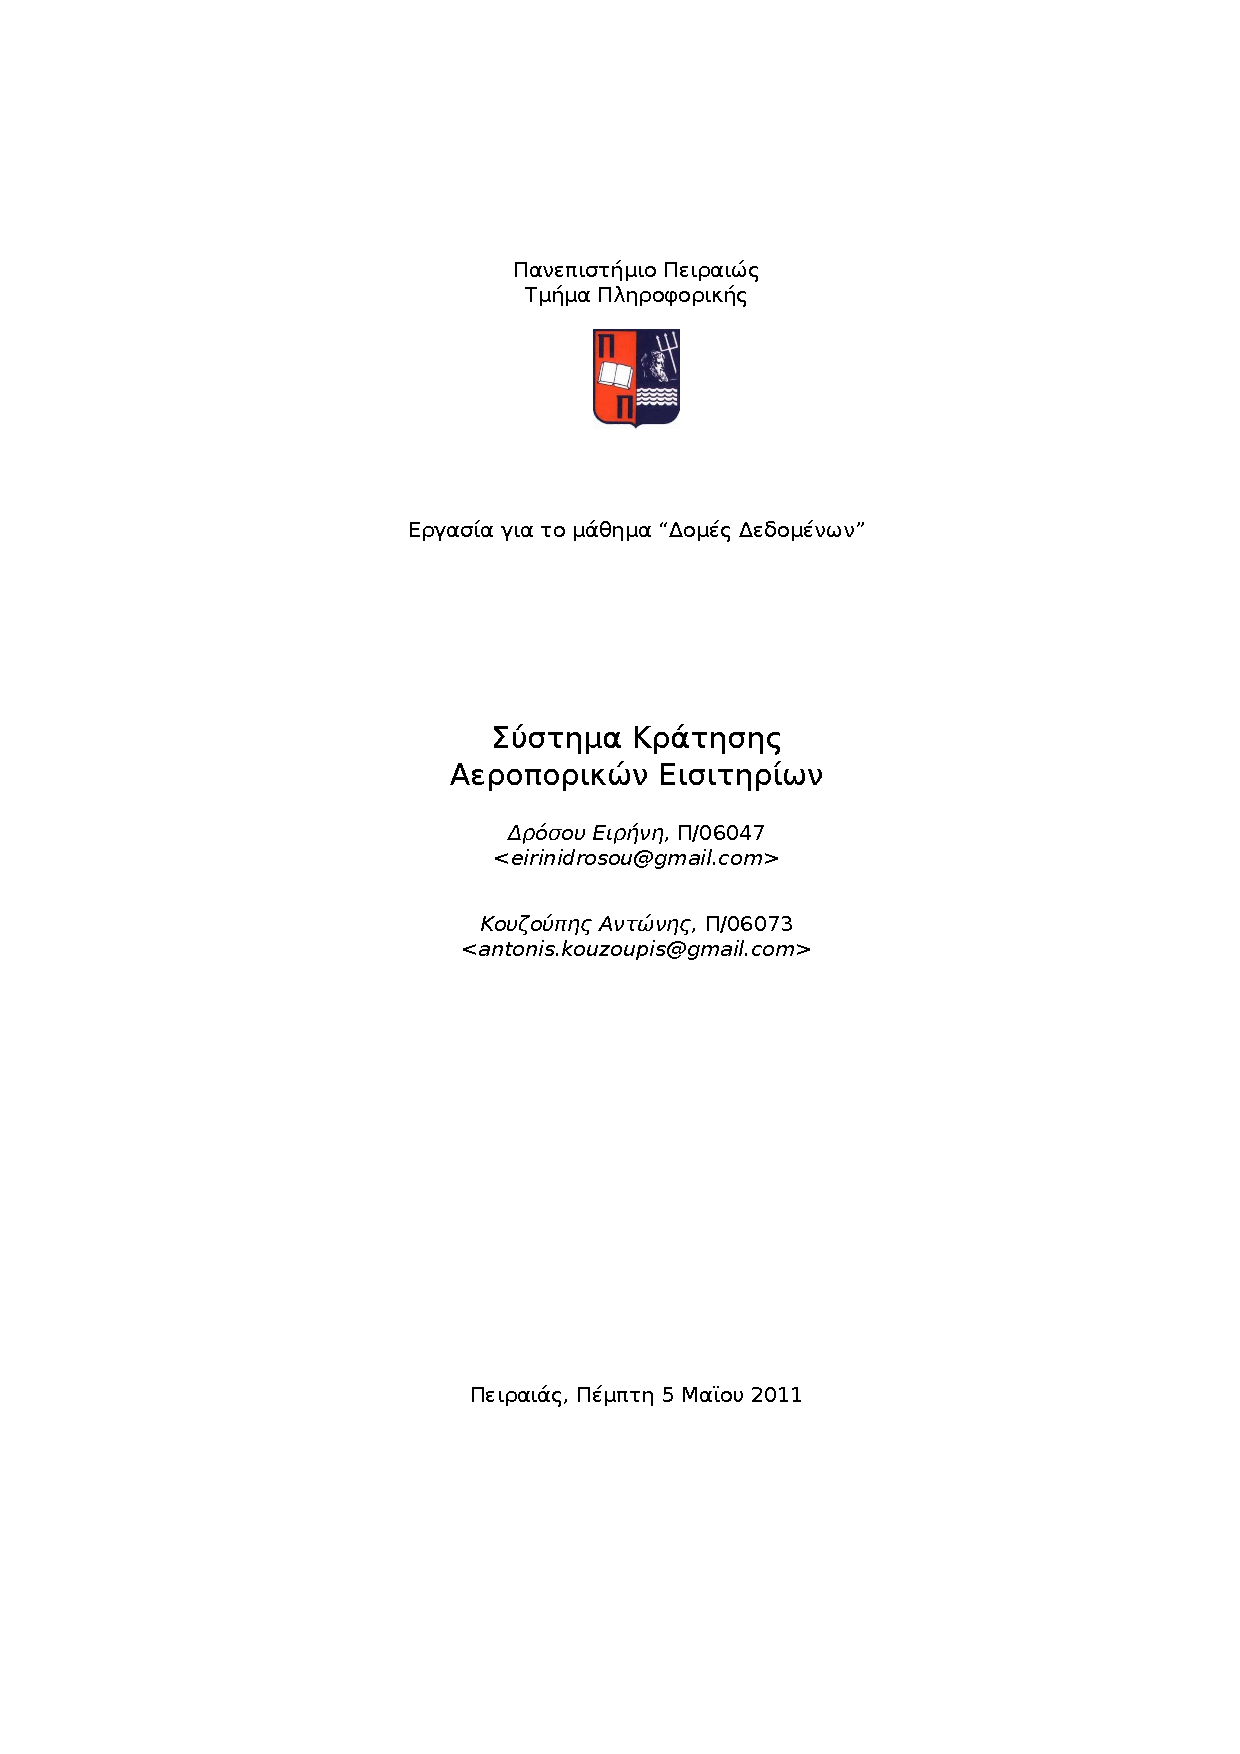
\includepdf[pages=-]{titlepage.pdf}
\tableofcontents
\newpage
\section{Εισαγωγή}
Η εφαρμογή υλοποιεί ένα απλοποιημένο σύστημα κράτησης αεροπορικών εισιτηρίων
Είναι γραμμένο στη γλώσσα προγραμματισμού Java. Οι δομές δεδομένων που
χρησιμοποιήθηκαν δεν είναι οι έτοιμες δομές που προσφέρει η γλώσσα. Η εφαρμογή
υποστηρίζει την προβολή, εισαγωγή και διαγραφή μιας πτήσης και τις αντίστοιχες
για τις κρατήσεις των επιβατών. Δεν χρησιμοποιεί κάποια τεχνολογία για
persistance καθώς δεν απαιτούνταν από την εργασία.

\section{Σχεδίαση}
Ο κώδικας της εφαρμογής είναι χωρισμένος σε τρία βασικά κομμάτια. Το κάθε
κομμάτι περιέχει κώδικα ``ανεξάρτητο'' από τα άλλα δύο. Παρόλα αυτά δεν είναι
κανένα αυτόνομο. Τα τρία directories--packages είναι τα \emph{business,
entities} και \emph{structures}. Το πρώτο package περιέχει όλο το business logic
της εφαρμογής. Δηλαδή περιέχει κλάσεις και μεθόδους που προσθέτει κάποιος μια
νέα πτήση, νέο επιβάτη κτλ. Το δεύτερο πακέτο αποτελείται από τις δύο οντότητες
της εφαρμογής, τους επιβάτες και τις πτήσεις. Οι κλάσεις αυτές είναι υπεύθυνες
για την αποθήκευση κρίσιμων πληροφοριών όπως Όνομα, Επίθετο κτλ για τους
επιβάτες και αριθμό πτήσης, ώρα αναχώρησης κτλ για τις πτήσεις. Το τρίτο και
τελευταίο κομμάτι έχει τις δομές δεδομένων που χρησιμοποιούμε στην εφαρμογή.
Συγκεκριμένα έχουμε υλοποιήσει μονά συνδεδεμένη λίστα, διπλά συνδεδεμένη λίστα
και ουρά αναμονής. Αναλυτική περιγραφή υπάρχει σε παρακάτω κεφάλαια.


\subsection{business package}
Το πακέτο αυτό περιέχει τις κλάσεις \emph{FlightsBusiness, Main,
PassengerBusiness} και \emph{Utilities}.

Η πρώτη κλάση έχει μεθόδους για τη δουλεία που γίνεται στη μεριά των πτήσεων.
Συγκεκριμένα διαχειρίζεται τη προ--φόρτωση κάποιων πτήσεων στο σύστημα, την
προβολή όλων των πτήσεων που είναι αποθηκευμένες στην εφαρμογή, την προσθήκη
νέων πτήσεων, τη διαγραφή πτήσεων, τη κράτηση πτήσεων από τους χρήστες, τον
έλεγχο της διαθεσιμότητας μιας πτήσης και τον έλεγχο των στοιχείων μιας
κράτησης.

Η δεύτερη κλάση αρχικοποιεί τις κατάλληλες δομές, τυπώνει το κεντρικό μενού και
αναλόγως την επιλογή καλεί τις κατάλληλες μεθόδους. Οι διαθέσιμες επιλογές του
χρήστη είναι η προβολή των διαθέσιμων πτήσεων, η προσθήκη μιας νέας πτήσης στο
σύστημα, η διαγραφή μιας πτήσης, η προσθήκη--κράτηση μιας κράτησης από τον
χρήστη, η προβολή όλων των επιβατών που έχουν καταχωρηθεί στην εφαρμογή, η
διαγραφή ενός επιβάτη και της κράτησής του και η έξοδος από την εφαρμογή.

Τρίτη κλάση είναι η \emph{PassengerBusiness} η όποια είναι υπεύθυνη για τις
λειτουργίες που αφορούν τους χρήστες. Χρησιμοποιείται για να εκτύπωση όλων των
επιβατών στο σύστημα, την εκτύπωση των κατάλληλων ``ερωτήσεων'' κατά την
εισαγωγή ενός νέου επιβάτη, για την εισαγωγή ενός νέου επιβάτη--κράτησης και για
την διαγραφή μιας κράτησης.

Τέλος η κλάση \emph{Utilities} περιέχει δύο βοηθητικές μεθόδους. Η πρώτη είναι
μία υλοποίηση της συνάρτησης κατακερματισμού md5 και η άλλη είναι η μετατροπή
μιας συμβολοσειράς σε δεκαεξαδική μορφή. Η τελευταία χρησιμοποιείται από την
μέθοδο που υλοποιεί το md5 hash.

\subsection{entities package}
Το πακέτο \emph{entities} περιέχει τις κλάσεις \emph{Flight} και
\emph{Passenger}.

Η κλάση \emph{Flight} είναι υπεύθυνη για την αποθήκευση όλων των στοιχείων
μιας πτήσης. Συγκεκριμένα τα στοιχεία που κρατάει είναι ο κωδικός πτήσης, την
αφετηρία, τον προορισμό, την ώρα αναχώρησης, την ώρα άφιξης, τη τιμή των
εισιτηρίων, τον τύπο του αεροσκάφους, των συνολικό αριθμό θέσεων στο αεροπλάνο,
τις διαθέσιμες θέσεις στο αεροπλάνο, τους επιβάτες που έχουν κάνει κράτηση για
τη συγκεκριμένη πτήση και υπάρχει θέση στο αεροπλάνο και τους επιβάτες οι οποίοι
έχουν κάνει κράτηση για τη συγκεκριμένη πτήση αλλά δεν υπάρχουν διαθέσιμες
θέσεις οπότε μπαίνουν σε λίστα αναμονής. Οι μέθοδοι που υπάρχουν είναι για να
θέτουμε μία νέα τιμή στις παραπάνω μεταβλητές και για να παίρνουμε τις τιμές των
παραπάνω μεταβλητών (getters \& setters). Επίσης υπάρχει και μία μέθοδος για την
εκτύπωση όλων των παραπάνω λεπτομερειών.

Η κλάση αυτή είναι υπεύθυνη για την αποθήκευση των λεπτομερειών ενός χρήστη
και της κράτησής του. Τα στοιχεία που κρατάει είναι το επίθετο, το όνομα, τον
αριθμό ταυτότητας, την εθνικότητα, τη διεύθυνση, το τηλέφωνο, το μοναδικό αριθμό
κράτησης του χρήστη, την κατάσταση της κράτησής του και μία λίστα με τους
κωδικούς πτήσης των δρομολογίων που έχει κάνει κράτηση. Οι μέθοδοι που υπάρχουν
στη κλάση αυτή είναι για να ορίζουμε μία νέα τιμή στα παραπάνω στοιχεία και για
να παίρνουμε την υπάρχουσα τιμή τους. Υπάρχει και μία μέθοδος για την εκτύπωση
όλων των παραπάνω στοιχείων.

\subsection{structures package}
Το πακέτο αυτό περιέχει τις κλάσεις \emph{DoublyLinkedList, FifoQueue} και
\emph{SimplyLinkedList}.

Η κλάση \emph{DoublyLinkedList} υλοποιεί τη διπλά συνδεδεμένη λίστα που
χρησιμοποιείται στην εφαρμογή. Χρησιμοποιεί τα Generics της Java για τον
προσδιορισμό του τύπου των στοιχείων που θα κρατάει. Αποτελείται από δύο
κλάσεις, την \emph{DNode} που κρατάει τις πληροφορίες για κάθε κόμβο όπως την
τιμή του κόμβου, τον επόμενο και τον προηγούμενο κόμβο καθώς και κάποιες
μεθόδους για την προσπέλαση των παραπάνω στοιχείων. Η δεύτερη κλάση είναι η
\emph{DoublyLinkedList} που υλοποιεί κάποιες λειτουργίες της διπλά συνδεδεμένης
λίστας όπως την διαγραφή ενός κόμβου ενώ παίρνουμε και την τιμή του, την
προσθήκη σε κάποια συγκεκριμένη θέση στη λίστα, την προσθήκη ενός κόμβου στην
αρχή, στο τέλος, μία μέθοδος για να παίρνουμε το μέγεθος της λίστας, μία για να
ξέρουμε αν η λίστα είναι άδεια και μία για να τυπώνουμε όλα τους κόμβους της
λίστας.

Η κλάση \emph{FifoQueue} υλοποιεί μία FIFO (First In First Out) ουρά αναμονής
βασισμένη σε μία απλά συνδεδεμένη λίστα. Χρησιμοποιεί επίσης τα Generics της
Java. Έχει δύο κλάσεις, η μία είναι η \emph{QNode} όπου κρατάει τα στοιχεία ενός
κόμβου όπως την τιμή του κόμβου και τον επόμενο κόμβο. Επίσης έχει κάποιες
μεθόδους για την προσπέλαση των στοιχείων αυτών. Τέλος η κλάση \emph{FifoQueue}
περιέχει μεθόδους για τις βασικές λειτουργίες της ουράς όπως είναι η εισαγωγή
στο τέλος, η εξαγωγή από την αρχή, η διαγραφή ενός στοιχείου στο ενδιάμεσο της
ουράς, μέθοδος για να παίρνουμε το μέγεθος της ουράς, για να βλέπουμε αν είναι
άδεια και μία μέθοδος για να τυπώνει τις τιμές των κόμβων της ουράς αναμονής.

Τέλος η κλάση \emph{SimplyLinkedList} υλοποιεί μία μονά συνδεδεμένη λίστα που
επίσης χρησιμοποιεί Generics. Αποτελείται και αυτή από δύο κλάσεις, η μία είναι η
\emph{SNode} που κρατάει διάφορες πληροφορίες για ένα κόμβο όπως τη τιμή του
κόμβου και τον επόμενο κόμβο. Έχει επίσης κάποιες μεθόδους για την προσπέλαση
των στοιχείων αυτών. Η κλάση \emph{SimplyLinkedList} υλοποιεί κάποιες
λειτουργίες της μονά συνδεδεμένης λίστας όπως την προσθήκη ενός κόμβου είτε στην
αρχή, είτε στο τέλος είτε κάπου ενδιάμεσα, τη διαγραφή ενός κόμβου, μέθοδο για
την παίρνουμε το μέγεθος της λίστας, μέθοδο για να βλέπουμε αν η λίστα είναι
άδεια και μία μέθοδο που τυπώνει τις τιμές όλων των κόμβων της λίστας.

\subsection{Δομή Εφαρμογής}
Pos leitourgei xontrika h efarmogh, domes pou xrhsimopoih8hkan ktl
\end{document}
